\begin{figure}[H]
\centering
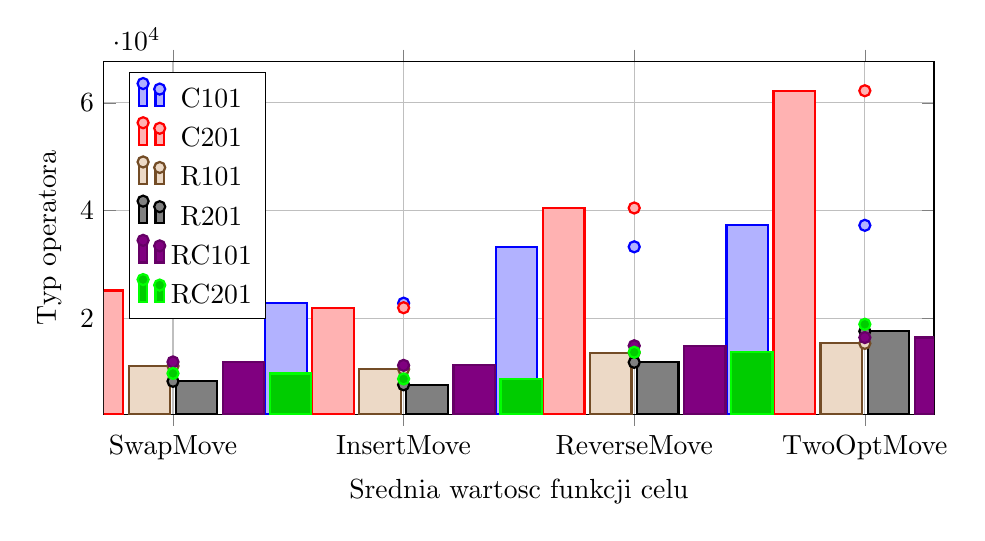
\begin{tikzpicture}
\begin{axis}[
xlabel = {Srednia wartosc funkcji celu},
ylabel = {Typ operatora},
legend pos = north west,
grid = both,
width=1\linewidth,
height=0.5\linewidth,
ybar,
bar width=15pt,
symbolic x coords={SwapMove,InsertMove,ReverseMove,TwoOptMove,},
xtick=data
]
\addplot + [mark = *, thick] coordinates
    {
(SwapMove,22709.333333333332)(InsertMove,22808.5)(ReverseMove,33274.333333333336)(TwoOptMove,37262.0)};
\addlegendentry
{C101}
\addplot + [mark = *, thick] coordinates
    {
(SwapMove,25147.666666666668)(InsertMove,21963.833333333332)(ReverseMove,40477.833333333336)(TwoOptMove,62244.166666666664)};
\addlegendentry
{C201}
\addplot + [mark = *, thick] coordinates
    {
(SwapMove,11145.166666666666)(InsertMove,10569.333333333334)(ReverseMove,13614.333333333334)(TwoOptMove,15344.166666666666)};
\addlegendentry
{R101}
\addplot + [mark = *, thick] coordinates
    {
(SwapMove,8304.666666666666)(InsertMove,7660.5)(ReverseMove,11827.0)(TwoOptMove,17601.166666666668)};
\addlegendentry
{R201}
\addplot + [mark = *, thick] coordinates
    {
(SwapMove,11899.833333333334)(InsertMove,11267.5)(ReverseMove,14904.666666666666)(TwoOptMove,16433.0)};
\addlegendentry
{RC101}
\addplot + [mark = *, thick] coordinates
    {
(SwapMove,9769.833333333334)(InsertMove,8749.166666666666)(ReverseMove,13698.0)(TwoOptMove,18891.0)};
\addlegendentry
{RC201}
\end{axis}
\end{tikzpicture}
\caption
{Srednia wartosc funkcji celu w zaleznosci od typu operatora dla poszczegolnych instancji}
\label{fig:mean_goals_per_bee_operator_per_instance}
\end{figure}
